\section{Introducción}
El análisis de Fourier es una familia de técnicas matemáticas, basadas en la descomposición de señales en señales sinusoidales. La Transformada Discreta de Fourier (TDF) es un miembro de esta familia la cual es usada para trabajar con señales digitales.\\ El objetivo de la descomposición de la señal es obtener algo más sencillo con lo cual trabajar (en este caso, con senos y cosenos) que lo que se tenia originalmente.\\ Para el tratamiento de señales discretas  se usa la TDF, la cual esta definida en la Figura 1:
\begin{figure}[H]
	\centering
	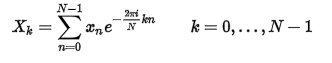
\includegraphics[scale=.8]{img/tdf.png}
	\caption{Transformada Discreta de Fourier}
	\label{fig:prub1}		
\end{figure}
Al usar la identidad de Euler (Figura 2) se puede obtener otra versión de la TDF donde la parte real este contenida en una sumatoria de cosenos y la parte imaginaria contenida en una sumatoria de senos.
\begin{figure}[H]
	\centering
	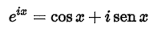
\includegraphics[scale=.8]{img/euler.png}
	\caption{Identidad de Euler}
	\label{fig:prueb1}		
\end{figure}
Lo cual se puede apreciar en la siguiente figura:
\begin{figure}[H]
	\centering
	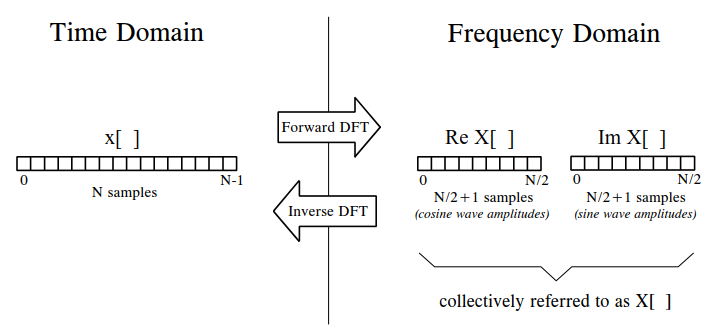
\includegraphics[scale=.7]{img/real.png}
	\caption{Parte Real e Imaginaria de la TDF}
	\label{fig:prue1}		
\end{figure}
Para este trabajo, cada una de las partes de la TDF (real e imaginaria) serán contenidas en un canal de un archivo wav, canal izquierdo para la parte real y canal derecho para la parte imaginaria. Por lo cual, como entrada para el programa de la TDF se recibirá un archivo de un canal (muestras de la señal discreta) y se obtendrá como salida un archivo wav de dos canales, donde el archivo de salida tendrá el mismo número de muestras que el archivo de entrada, pero el tamaño de las mismas ahora será de 4 bytes (2 bytes por el canal izquierdo y 2 bytes por el canal derecho).\\ 
Así como fue realizada la práctica del reporte 01A donde se simulaba un circuito RC (filtro pasabajas) mediante el uso de la convolución, en esta práctica se busca simular lo mismo, pero en lugar de usar la convolución, se usará el producto en frecuencia, lo cual es equivalente a realizar la convolución en el tiempo. Para realizar ese procedimiento, es necesario primero aplica la TDF a la señal de entrada, y posteriormente la salida obtenida multiplicarla por el filtro ideal en frecuencia que se desarrolló.\\ Finalmente al resultado de la multiplicación es necesario ingresarlo al programa que calcula la TDF Inversa, la cual regresa al dominio del tiempo una señal que se encuentra en el dominio de la frecuencia (en este caso, el archivo que fue resultado de la multiplicación).\\ Cabe señalar, que el programa que calcula la TDF tiene 4 modos de ejecución, donde además de obtener la TDF se puede obtener otra información importante como la magnitud y fase de la transformada.
